\documentclass[t]{beamer}
\usetheme[deutsch]{KIT}
\setbeamercovered{transparent}
\setbeamertemplate{navigation symbols}{}

\KITfoot{YUV.KA - Praxis der Softwareentwicklung WS 11/12}
\usepackage[utf8]{inputenc}
\usepackage{ngerman}
\usenavigationsymbols

\title{YUV.KA}
\subtitle{PSE - Abschlusspräsentation \\[0.3cm]
Max Wagner $\cdot$ Patrick Gemander $\cdot$ Sebastian Ullrich $\cdot$ Michael Vollmer \\ Robert Hangu $\cdot$ Daniel Lebert}

\institute[ITEC]{Institut für Technische Informatik}

\TitleImage[trim = -20cm 0 0 0,height=\titleimageht]{logo.png}

\AtBeginSection[]
{
  \begin{frame}
    \frametitle{Übersicht}
    \tableofcontents[currentsection]
  \end{frame}
}

\begin{document}

\begin{frame}
	\maketitle
\end{frame}

\begin{frame}
	\frametitle{Übersicht}
	\addcontentsline{toc}{section}{}
	\tableofcontents
\end{frame}

\section{Vorwissen}
\begin{frame}
	\frametitle{Was ist ein Videoencoder?}
	\begin{center}
		\vspace*{\fill}
		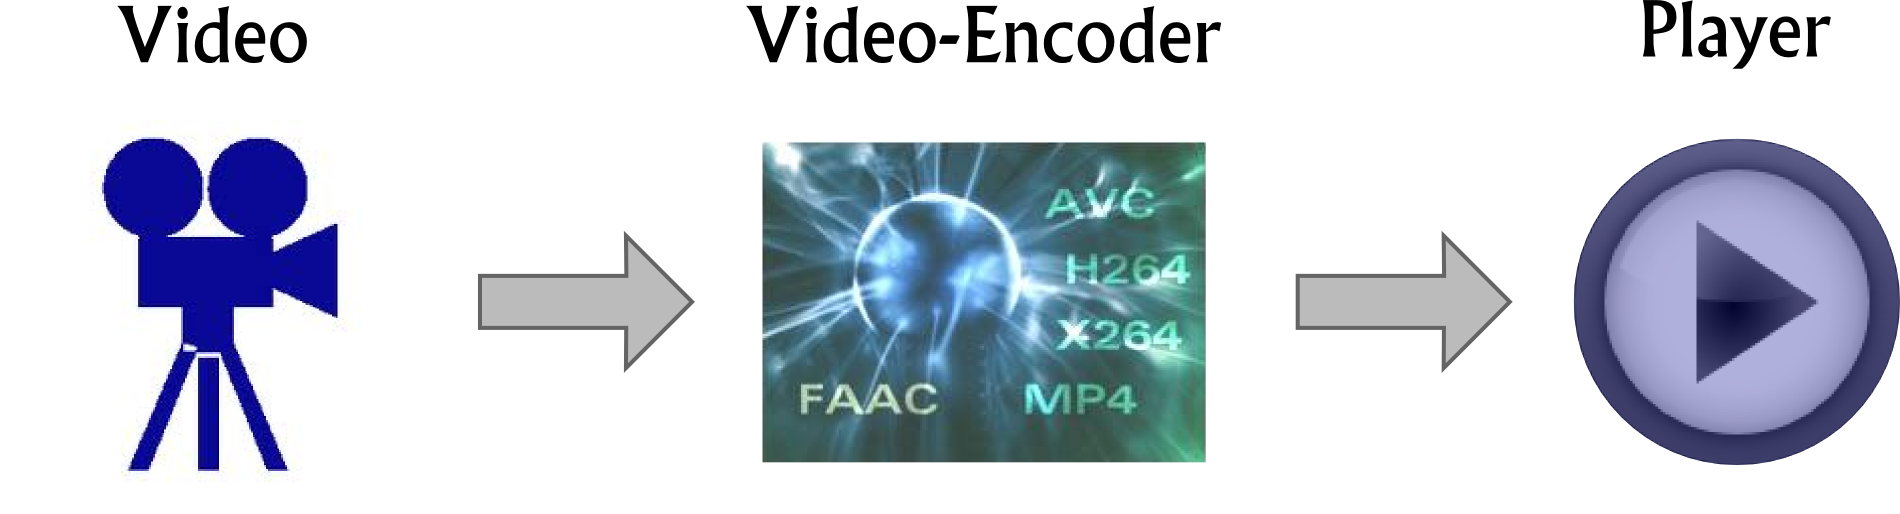
\includegraphics[scale=.43]{video-encoding-process.png}
		\vspace*{\fill}
		\onslide<2-> Warum das Ganze? ~\\
		\onslide<3-> $ \Longrightarrow $ Speicherbedarf der Videos reduzieren
	\end{center}
\end{frame}

\begin{frame}
	\frametitle{Funktionsweise des Encoders}
	\begin{minipage}{5.5cm}
		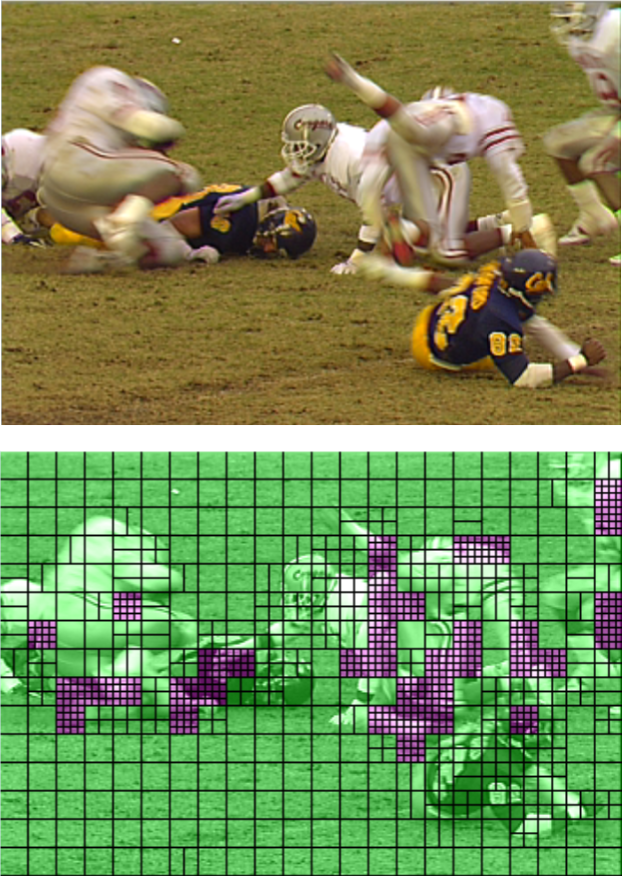
\includegraphics[scale=.29]{overlay-medium.png}	
	\end{minipage}
	\begin{minipage}{5.5cm}
		\begin{itemize}
			\item<+-> Unterteilung in Makroblöcke
			\item<+-> Wiederverwendung von Bildteilen aus dem aktuellen Frame
			\item<+-> Wiederverwendung von Bildteilen aus vorherigen Frames
		\end{itemize}
	\end{minipage}
\end{frame}

\begin{frame}
	\frametitle{Der Referenzencoder}
	~\\
	% Referenz-Encoder
	\begin{minipage}{5.3cm}
		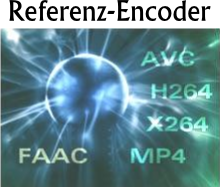
\includegraphics[scale=.5]{ref.png}
		~\\
		\begin{itemize}
			\item<2-> Liefert optimale Lösung
			\item<4-> Geht alle Möglichkeiten durch
		\end{itemize}
		\onslide<5->{ $ \Longrightarrow $ Extrem langsam}
	\end{minipage}
	\hfill	
	% Beliebiger Encoder
	\begin{minipage}{4.7cm}
		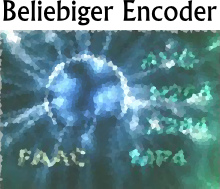
\includegraphics[scale=.5]{beliebig.png}
		~\\
		\begin{itemize}
			\item<3-> Liefert meist gute Lösung
			\item<6-> Heuristisches Vorgehen			
		\end{itemize}
		\onslide<7->{ $ \Longrightarrow $ Deutlich schneller }
	\end{minipage}
\end{frame}

\section{Das Projekt}
\begin{frame}
	\frametitle{Das Projekt}
	\begin{center}
		Ein Multimedia-Framework zur Evaluierung von Videoencodern	
	\end{center}
	\onslide<2->{ Was ist dazu nötig? } \newline
	\begin{itemize}
		\item<3-> Videos im YUV-Format einlesen und manipulieren
	\end{itemize}
	~\\
	~\\
	~\\
	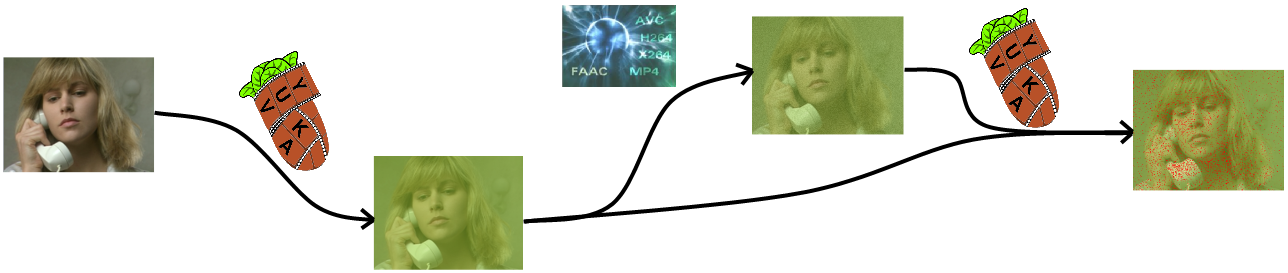
\includegraphics[scale=.34]{YuvKA-Workchart.png}
\end{frame}

\begin{frame}
	\frametitle{Beispiel}

	\begin{center}
		Original ~\\
		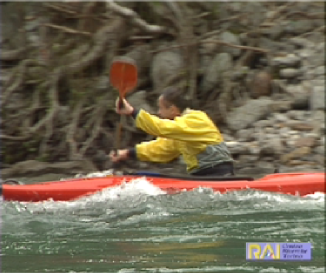
\includegraphics[scale=.45]{rafting-original.png}	
	\end{center}
	\begin{minipage}{5cm}
		\begin{center}
			Verschwommenes Bild ~\\
			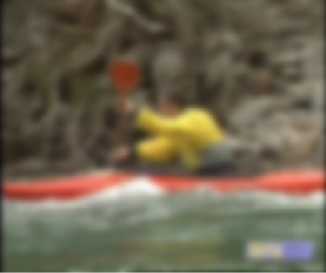
\includegraphics[scale=.45]{rafting-blur.png}		
		\end{center}	
	\end{minipage}
	\hfill
	\begin{minipage}{5cm}
		\begin{center}
			Bild mit Grünstich ~\\
			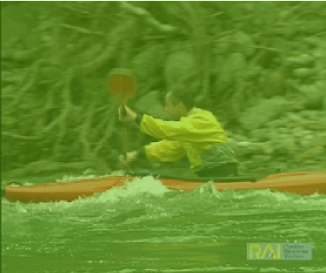
\includegraphics[scale=.45]{rafting-green.png}
		\end{center}	
	\end{minipage}
	\hfill
\end{frame}

\begin{frame}
	\frametitle{Das Projekt}
	\begin{center}
		Ein Multimedia-Framework zur Evaluierung von Videoencodern	
	\end{center}
	\onslide<1-> Was ist dazu nötig? \newline
	\begin{itemize}
		\item<1-> Videos im YUV-Format einlesen und manipulieren
		\item<2-> Videos mit einem externen Encoder encodieren
		\item<3-> Ergebnisse mit Hilfe des Programms analysieren
	\end{itemize}
	~\\
	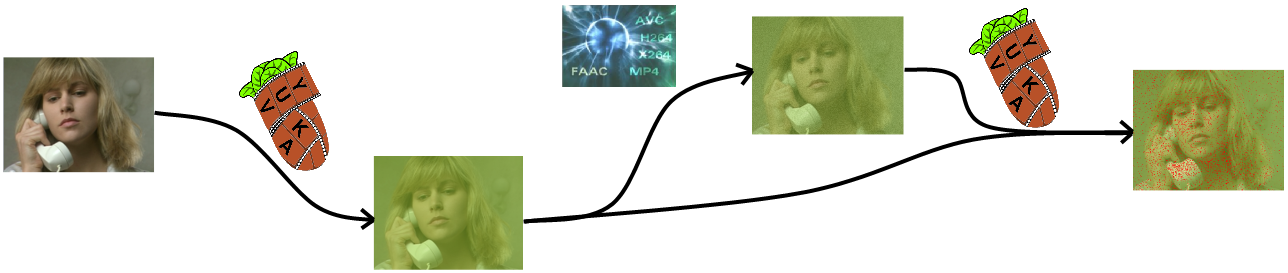
\includegraphics[scale=.34]{YuvKA-Workchart.png}
\end{frame}

\begin{frame}
	\frametitle{Beispiel}

	\begin{center}
		Original ~\\
		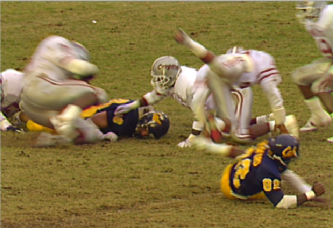
\includegraphics[scale=.2]{football-original.png}	
	\end{center}
	\begin{minipage}{5cm}
		\begin{center}
			Bild mit Makroblock-Overlay ~\\
			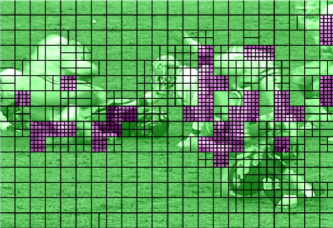
\includegraphics[scale=.2]{football-macroblock.png}		
		\end{center}	
	\end{minipage}
	\hfill
	\begin{minipage}{5cm}
		\begin{center}
			Bild mit Artefakt-Overlay ~\\
			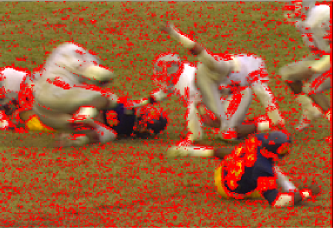
\includegraphics[scale=.455]{football-artifact.png}
		\end{center}	
	\end{minipage}
	\hfill
\end{frame}


\begin{frame}
	\frametitle{Das Projekt}
	\begin{center}
		Ein Multimedia-Framework zur Evaluierung von Videoencodern	
	\end{center}
	\onslide<1-> Was ist dazu nötig? \newline
	\begin{itemize}
		\item<1-> Videos im YUV-Format einlesen und manipulieren
		\item<1-> Videos mit einem externen Encoder encodieren
		\item<1-> Ergebnisse mit Hilfe des Programms analysieren
	\end{itemize}
	\onslide<2>{$ \Longrightarrow $ Programm soll Forschern beim Testen ihrer Encoder helfen}
	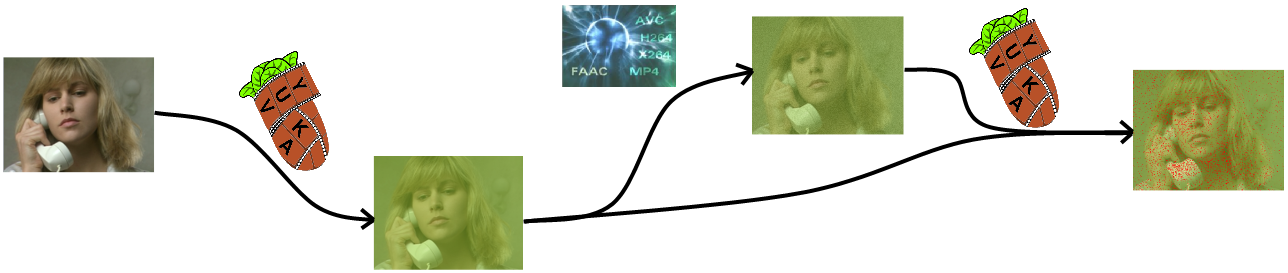
\includegraphics[scale=.34]{YuvKA-Workchart.png}
\end{frame}

\section{Unsere Lösung}
\begin{frame}
	\frametitle{Die Lösung: YUV.KA}
	\begin{center}
		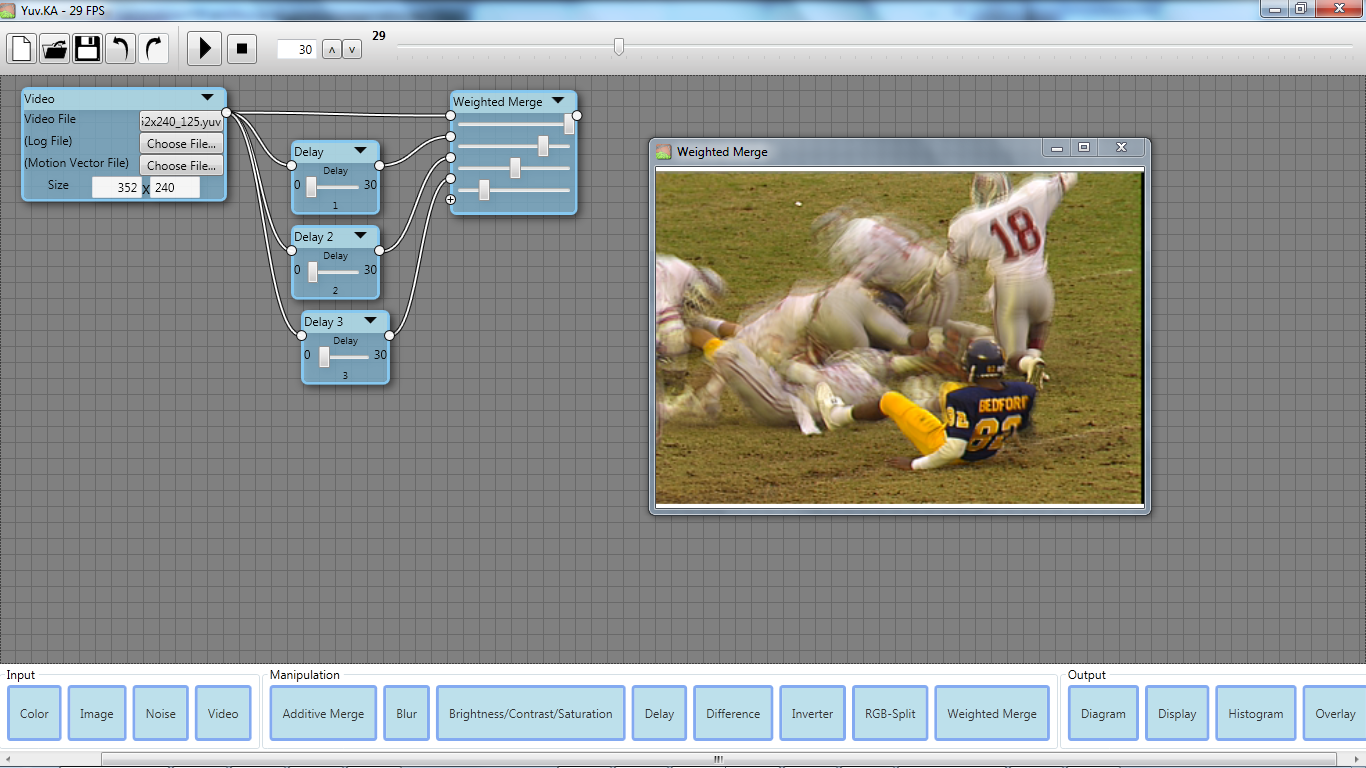
\includegraphics[height=.9\textheight]{startup_screenshot.png}
	\end{center}
\end{frame}

\begin{frame}
	\frametitle{Entwurf I}
	
	Entwicklungsumgebung ~\\
	\begin{itemize}
		\item<+-> C\#
		\item<+-> WPF (\textbf{W}indows \textbf{P}resentation \textbf{F}oundation)
		\item<+-> Microsoft Visual Studio 2010
	\end{itemize}
\end{frame}

\begin{frame}
    \frametitle{Benutzte Frameworks}
    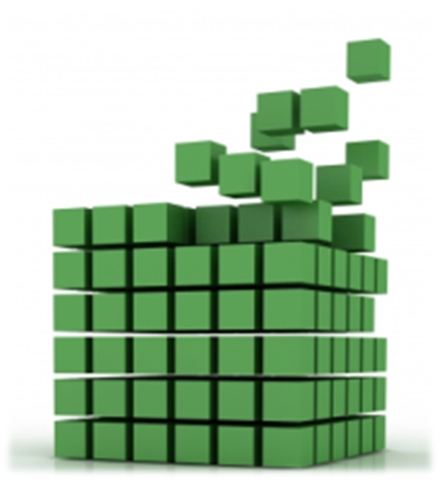
\includegraphics[scale=0.1]{img/mef} \hspace{0.1cm}
    
\includegraphics[scale=0.4]{img/d3} \hspace{0.1cm}
    
\includegraphics[scale=0.4]{img/td} \hspace{0.5cm}
    
\includegraphics[scale=0.4]{img/caliburn} ~\\
    \vspace{0.5} \hspace{0.6cm} 
\includegraphics[scale=0.45]{img/xunit} \hspace{0.7cm}
    
\includegraphics[scale=0.6]{img/moq}~\\
    \vspace{0.5cm} \hspace{0.5cm} 
\includegraphics[scale=0.24]{img/net} \hspace{0.8cm}
    
\includegraphics[scale=0.6]{img/rx}

\end{frame}

\begin{frame}
	\frametitle{Entwurf II}
	\noindent
	\begin{minipage}{3.5cm}
	    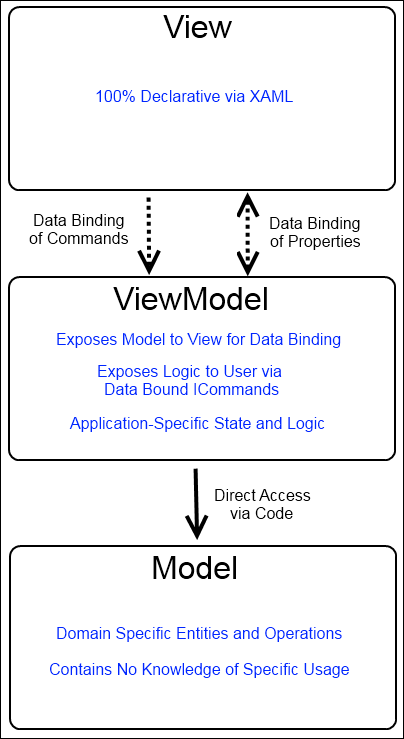
\includegraphics[width=3.5cm]{MVVM_thumb.png} ~\\
	    \textit{http://reedcopsey.com}
	\end{minipage}
	\hfill
	\begin{minipage}{8cm}
		Architektur - MVVM-Entwurfsmuster ~\\
	    \begin{itemize}	    
	    	\item<+-> Model-View-ViewModel
	        \item<+-> Eigens für WPF entwickeltes Entwurfsmuster
	        \item<+-> Erzielt Modularität und Testbarkeit durch vollständige Entkopplung von UI-Elementen und UI-Logik
	    \end{itemize}
	\end{minipage}
\end{frame}

\begin{frame}
    \frametitle{Das Testen}
    \vspace{1cm}
	\begin{tabular}{@{\extracolsep{\fill}} |l|c|}
		\hline
		Namespace &  Überdeckung in \% \\ \hline
		YuvKA.Pipeline  &  98,32  \\ \hline
		YuvKA.VideoModel  & 86,50 \\ \hline
		YuvKA.ViewModel  & 92,77  \\ \hline
		YuvKA.ViewModel.PropertyEditor  & 98,15  \\ \hline
		YuvKA.Implementation  &  72,15 \\ \hline
		YuvKA.Pipeline.Implementation  &  92,39  \\ \hline
		YuvKA.ViewModel.Implementation  & 84,70 \\ \hline
		YuvKA.ViewModel.PropertyEditor.Implementation  & 76,28  \\ \hline
		\hline
		\textbf{Overall} & \textbf{90,79} \\ \hline
	\end{tabular}
	~\\
	Zeilen eigener Code insgesamt: ca. 7300 ~\\ % actual 7318   
	Zeilen Testcode insgesamt: ca. 3900    % actual 3860
\end{frame}

\begin{frame}
    \frametitle{Erkenntnisse aus dem Projekt}
    \begin{itemize}
        \item<+-> Entwurf vor Implementierung funktioniert...
        \item<+-> ... kann jedoch Probleme mit sich bringen
        \item<+-> Kommunikation und Koordination sind essentiell
        \item<+-> Softwareentwicklung ist sehr zeitintensiv
        \item<+-> (Graphische) Benutzeroberfläche benötigt (wesentlich) mehr Aufwand als Programmlogik
    \end{itemize}
\end{frame}

\section{Live-Demo}
%\begin{frame}
%	\begin{center}
%		\textbf{Live-Demo}
%	\end{center}
%\end{frame}

\end{document} 
